
\documentclass[11pt,a4paper]{CLabBookTemplate} %load the style file for the Extended Essay

\addbibresource{MyBibliography.bib} %specifying the bibliography file

% information about you and the document
\author{Tim Meiwald}
 %000017-0104 -> candidate number
\usepackage{multicol}


% For the C code snippets
\usepackage{listings}
\usepackage{xcolor}
\usepackage{mhchem}
\usepackage[utf8]{inputenc}
\definecolor{mGreen}{rgb}{0,0.6,0}
\definecolor{mGray}{rgb}{0.5,0.5,0.5}
\definecolor{mPurple}{rgb}{0.58,0,0.82}
\definecolor{backgroundColour}{rgb}{0.95,0.95,0.92}

\lstdefinestyle{CStyle}{
	backgroundcolor=\color{backgroundColour},   
	commentstyle=\color{mGreen},
	keywordstyle=\color{magenta},
	numberstyle=\tiny\color{mGray},
	stringstyle=\color{mPurple},
	basicstyle=\footnotesize,
	breakatwhitespace=false,         
	breaklines=true,                 
	captionpos=b,                    
	keepspaces=true,                 
	numbers=left,                    
	numbersep=5pt,                  
	showspaces=false,                
	showstringspaces=false,
	showtabs=false,                  
	tabsize=2,
	language=C
}

\lstdefinestyle{PythonStyle}{
	backgroundcolor=\color{backgroundColour},   
	commentstyle=\color{red},
	keywordstyle=\color{blue},
	numberstyle=\tiny\color{mGray},
	stringstyle=\color{mGreen},
	basicstyle=\footnotesize,
	breakatwhitespace=false,         
	breaklines=true,                 
	captionpos=b,                    
	keepspaces=true,                 
	numbers=left,                    
	numbersep=5pt,                  
	showspaces=false,                
	showstringspaces=false,
	showtabs=false,                  
	tabsize=2,
	language=Python
}

\lstset{language=C}

\lstset{literate=
	{á}{{\'a}}1 {é}{{\'e}}1 {í}{{\'i}}1 {ó}{{\'o}}1 {ú}{{\'u}}1
	{Á}{{\'A}}1 {É}{{\'E}}1 {Í}{{\'I}}1 {Ó}{{\'O}}1 {Ú}{{\'U}}1
	{à}{{\`a}}1 {è}{{\`e}}1 {ì}{{\`i}}1 {ò}{{\`o}}1 {ù}{{\`u}}1
	{À}{{\`A}}1 {È}{{\'E}}1 {Ì}{{\`I}}1 {Ò}{{\`O}}1 {Ù}{{\`U}}1
	{ä}{{\"a}}1 {ë}{{\"e}}1 {ï}{{\"i}}1 {ö}{{\"o}}1 {ü}{{\"u}}1
	{Ä}{{\"A}}1 {Ë}{{\"E}}1 {Ï}{{\"I}}1 {Ö}{{\"O}}1 {Ü}{{\"U}}1
	{â}{{\^a}}1 {ê}{{\^e}}1 {î}{{\^i}}1 {ô}{{\^o}}1 {û}{{\^u}}1
	{Â}{{\^A}}1 {Ê}{{\^E}}1 {Î}{{\^I}}1 {Ô}{{\^O}}1 {Û}{{\^U}}1
	{œ}{{\oe}}1 {Œ}{{\OE}}1 {æ}{{\ae}}1 {Æ}{{\AE}}1 {ß}{{\ss}}1
	{ű}{{\H{u}}}1 {Ű}{{\H{U}}}1 {ő}{{\H{o}}}1 {Ő}{{\H{O}}}1
	{ç}{{\c c}}1 {Ç}{{\c C}}1 {ø}{{\o}}1 {å}{{\r a}}1 {Å}{{\r A}}1
	{€}{{\euro}}1 {£}{{\pounds}}1 {«}{{\guillemotleft}}1
	{»}{{\guillemotright}}1 {ñ}{{\~n}}1 {Ñ}{{\~N}}1 {¿}{{?`}}1
}


\title{MA4080 - Computational Task 2 } % use capitals


% \component{Electronic Lab Book} % or Lab report, Exploration, etc
% \session{Year 1 Semester 1}

% \wordcount{xxxx} %change this to the actual number

\usepackage{graphicx}

\begin{document}

\pagenumbering{roman} %roman page numbers to be used on the title, abstract, acknowledgment and contents page
\setcounter{page}{1} % start with page 1

\maketitle % generating the title page




% Generating the table of contents
\thispagestyle{fancy} % put the required information in the header
\addcontentsline{toc}{section}{Contents} % include this in the table of contents
\mytableofcontents
\newpage % Start the main text on a new page


% Here comes the important part, the main text
\pagenumbering{arabic} % arabic page numbers to be used from now on
\setcounter{page}{1} % start again with page 1

\section{Introduction}
In this task we model a text similar to Claude Shannon and Markov, by evaluating how a text behaves using Markov chains where each character is a state that can transition into another state. Those states could be their value, such as "a" or their state in terms of whether they are a vowel or a consonant. In order to do this, we need a text, in order to ensure uniqueness I have selected "Sleeping Beauty" but the german text thereof. \\

The text is \\

"Vor Zeiten war ein König und eine Königin, die sprachen jeden Tag: "Ach, wenn wir doch ein Kind hätten!" und kriegten immer keins.

Da trug es sich zu, als die Königin einmal im Bade saß, daß ein Frosch aus dem Wasser ans Land kroch und zu ihr sprach: "Dein Wunsch wird erfüllt werden, ehe ein Jahr vergeht, wirst du eine Tochter zur Welt bringen."

Was der Frosch gesagt hatte, das geschah, und die Königin gebar ein Mädchen, das war so schön, daß der König vor Freude sich nicht zu fassen wußte und ein großes Fest anstellte. Er ladete nicht bloß seine Verwandten, Freunde und Bekannten, sondern auch die weisen Frauen dazu ein, damit sie dem Kind hold und gewogen wären. Es waren ihrer dreizehn in seinem Reiche, weil er aber nur zwölf goldene Teller hatte, von welchen sie essen sollten, so mußte eine von ihnen daheim bleiben.

Das Fest ward mit aller Pracht gefeiert, und als es zu Ende war, beschenkten die weisen Frauen das Kind mit ihren Wundergaben: die eine mit Tugend, die andere mit Schönheit, die dritte mit Reichtum und so mit allem, was auf der Welt zu wünschen ist. Als elfe ihre Sprüche eben getan hatten, trat plötzlich die dreizehnte herein.

Sie wollte sich dafür rächen, daß sie nicht eingeladen war, und ohne jemand zu grüßen oder nur anzusehen, rief sie mit lauter Stimme: "Die Königstochter soll sich in ihrem fünfzehnten Jahr an einer Spindel stechen und tot hinfallen." Und ohne ein Wort weiter zu sprechen kehrte sie sich um und verließ den Saal.

Alle waren erschrocken, da trat die zwölfte hervor, die ihren Wunsch noch übrig hatte, und weil sie den bösen Spruch nicht aufheben, sondern ihn nur mildern konnte, so sagte sie: "Es soll aber kein Tod sein, sondern ein hundertjähriger tiefer Schlaf, in welchen die Königstochter fällt.

Der König, der sein liebes Kind vor dem Unglück gern bewahren wollte, ließ den Befehl ausgehen, daß alle Spindeln im ganzen Königreiche sollten verbrannt werden. An dem Mädchen aber wurden die Gaben der weisen Frauen sämtlich erfüllt, denn es war so schön, sittsam, freundlich und verständig daß es jedermann, der es ansah, liebhaben mußte. Es geschah, daß an dem Tage, wo es gerade fünfzehn Jahre alt ward, der König und die Königin nicht zu Haus waren und das Mädchen ganz allein im Schloß zurückblieb. Da ging es allerorten herum, besah Stuben und Kammern, wie es Lust hatte, und kam endlich auch an einen alten Turm. Es stieg die enge Wendeltreppe hinauf und gelangte zu einer kleinen Türe. In dem Schloß steckte ein verrosteter Schlüssel, und als es ihn umdrehte, sprang die Türe auf, und da saß in einem kleinen Stübchen eine alte Frau mit einer Spindel und spann emsig ihren Flachs.

"Guten Tag, du altes Mütterchen", sprach die Königstochter, "was machst du da?"

"Ich spinne", sagte die Alte und nickte mit dem Kopf.

"Was ist das für ein Ding, das so lustig herumspringt?" sprach das Mädchen, nahm die Spindel und wollte auch spinnen. Kaum hatte sie aber die Spindel angerührt so ging der Zauberspruch in Erfüllung, und sie stach sich damit in den Finger.

In dem Augenblick aber, wo sie den Stich empfand, fiel sie auf das Bett nieder, das da stand, und lag in einem tiefen Schlaf. Und dieser Schlaf verbreitete sich über das ganze Schloß, der König und die Königin, die eben heimgekommen waren und in den Saal getreten waren, fingen an einzuschlafen und der ganze Hofstaat mit ihnen. Da schliefen auch die Pferde im Stall, die Hunde im Hof, die Tauben auf dem Dache, die Fliegen an der Wand, ja, das Feuer, das auf dem Herde flackerte, ward still und schlief ein, und der Braten hörte auf zu brutzeln, und der Koch, der den Küchenjungen, weil er etwas versehen hatte, an den Haaren ziehen wollte, ließ ihn los und schlief. Und der Wind legte sich, und auf den Bäumen vor dem Schloß regte sich kein Blättchen mehr.

Rings um das Schloß aber begann eine Dornenhecke zu wachsen, die jedes Jahr höher ward und endlich das ganze Schloß umzog und darüber hinauswuchs, daß gar nichts mehr davon zu sehen war, selbst nicht die Fahne auf dem Dach. Es ging aber die Sage in dem Land von dem schönen, schlafenden Dornröschen, denn so ward die Königstochter genannt, also daß von Zeit zu Zeit Königssöhne kamen und durch die Hecke in das Schloß dringen wollten. Es war ihnen aber nicht möglich, denn die Dornen, als hätten sie Hände, hielten fest zusammen, und die Jünglinge blieben darin hängen, konnten sich nicht wieder losmachen und starben eines jämmerlichen Todes.

Nach langen, langen Jahren kam wieder einmal ein Königssohn in das Land und hörte, wie ein alter Mann von der Dornenhecke erzählte, es sollte ein Schloß dahinter stehen, in welchem eine wunderschöne Königstochter, Dornröschen genannt, schon seit hundert Jahren schliefe, und mit ihr schliefe der König und die Königin und der ganze Hofstaat. Er wußte auch von seinem Großvater, daß schon viele Königssöhne gekommen wären und versucht hätten, durch die Dornenhecke zu dringen, aber sie wären darin hängengeblieben und eines traurigen Todes gestorben.

Da sprach der Jüngling: "Ich fürchte mich nicht, ich will hinaus und das schöne Dornröschen sehen !" Der gute Alte mochte ihm abraten, wie er wollte, er hörte nicht auf seine Worte.

Nun waren aber gerade die hundert Jahre verflossen, und der Tag war gekommen, wo Dornröschen wieder erwachen sollte. Als der Königssohn sich der Dornenhecke näherte, waren es lauter große, schöne Blumen, die taten sich von selbst auseinander und ließen ihn unbeschädigt hindurch, und hinter ihm taten sie sich wieder als eine Hecke zusammen. Im Schloßhof sah er die Pferde und scheckigen Jagdhunde liegen und schlafen, auf dem Dache saßen die Tauben und hatten das Köpfchen unter den Flügel gesteckt. Und als er ins Haus kam, schliefen die Fliegen an der Wand, der Koch in der Küche hielt noch die Hand, als wollte er den Jungen anpacken, und die Magd saß vor dem schwarzen Huhn, das sollte gerupft werden.

Da ging er weiter und sah im Saale den ganzen Hofstaat liegen und schlafen, und oben bei dem Throne lagen der König und die Königin.

Da ging er noch weiter, und alles war so still, daß er seinen Atem hören konnte, und endlich kam er zu dem Turm und öffnete die Türe zu der kleinen Stube, in welcher Dornröschen schlief.

Da lag es und war so schön, daß er die Augen nicht abwenden konnte, und er bückte sich und gab ihm einen Kuß. Wie er es mit dem Kuß berührt hatte, schlug Dornröschen die Augen auf, erwachte und blickte ihn ganz freundlich an.

Da gingen sie zusammen herab, und der König erwachte und die Königin und der ganze Hofstaat und sahen einander mit großen Augen an. Und die Pferde im Hof standen auf und rüttelten sich, die Jagdhunde sprangen und wedelten, die Tauben auf dem Dache zogen das Köpfchen unterm Flügel hervor, sahen umher und flogen ins Feld, die Fliegen an den Wänden krochen weiter, das Feuer in der Küche erhob sich, flackerte und kochte das Essen, der Braten fing wieder an zu brutzeln, und der Koch gab dem Jungen eine Ohrfeige, daß er schrie, und die Magd rupfte das Huhn fertig.

Und da wurde die Hochzeit des Königssohns mit dem Dornröschen in aller Pracht gefeiert, und sie lebten vergnügt bis an ihr Ende."



\newpage
\section{Task 1}
As we can clearly see in order to do an analysis we will want to clean the data by stripping out punctuation, removing any whitespaces other than spaces and removing capitalization for easier analysis. Additionally we want to know the length of the text and the number of vowels and consonants. To be exact, the length of the text is after the punctuation and whitespace has been stripped. We can do this simply with python . To note, the Vowels and Consonants in German differ from that of English because of additional possible characters. 

\lstinputlisting[language=Python,style = PythonStyle,firstline = 48,lastline = 85]{Code/Code.py}
\begin{gather}
	\textrm{Length} = 6900 \\
	\textrm{Vowels} = 2098\\
	\textrm{Consonants} = 3553\\
	\textrm{Number of Spaces} = 1215 \\
	\textrm{Number of Stripped Symbols} = 201 
\end{gather}
\newpage


\section{Task 2}
We can find the probability of any character being followed by another character by using \eqref{TransitionProbability}.
\begin{equation}
	\label{TransitionProbability}
	\textrm{For any A} \rightarrow \textrm{B}, P_{t} = P(B|A) = \frac{P(B \cap A)}{P(B)} 
\end{equation}
We can do this using this code. 
\lstinputlisting[language=Python,style = PythonStyle,firstline = 86,lastline = 117]{Code/Code.py}
This first cleans up the text then counts the transition probability for each character followed by every other character and returns the result as a 2D array. To note, the final "character" checked for it's probability is a space because if we do so then we should end up with a right stochastic matrix. I.e the sum of all rows should equal 1. Unfortunately, it doesn't always equal 1, possibly due to round off error. Since some characters occur orders of magnitude more frequently than others, then the sum will lose precision because of the finite precision machine used to calculate it. \\


\begin{table}[htbp]
	\centering
	\caption{Part 1 of Probability Transition Matrix. N.b x1Ex2 represents x1 $\times$ $10^{x2}$}
	\begin{tabular}{lrrrrrrrr}
		Row $\rightarrow$ Col & \multicolumn{1}{l}{a} & \multicolumn{1}{l}{ä} & \multicolumn{1}{l}{b} & \multicolumn{1}{l}{c} & \multicolumn{1}{l}{d} & \multicolumn{1}{l}{e} & \multicolumn{1}{l}{ë} & \multicolumn{1}{l}{f} \\
		a     & 2.25E-02 & 0.00E+00 & 5.06E-02 & 6.74E-02 & 1.40E-02 & 0.00E+00 & 0.00E+00 & 2.25E-02 \\
		ä     & 0.00E+00 & 0.00E+00 & 0.00E+00 & 4.00E-02 & 2.00E-01 & 0.00E+00 & 0.00E+00 & 0.00E+00 \\
		b     & 2.63E-02 & 1.32E-02 & 0.00E+00 & 1.32E-02 & 0.00E+00 & 5.39E-01 & 0.00E+00 & 0.00E+00 \\
		c     & 0.00E+00 & 0.00E+00 & 0.00E+00 & 0.00E+00 & 0.00E+00 & 0.00E+00 & 0.00E+00 & 0.00E+00 \\
		d     & 1.59E-01 & 0.00E+00 & 0.00E+00 & 1.01E-02 & 0.00E+00 & 3.32E-01 & 0.00E+00 & 0.00E+00 \\
		e     & 0.00E+00 & 0.00E+00 & 1.23E-02 & 1.23E-02 & 1.12E-02 & 0.00E+00 & 0.00E+00 & 1.45E-02 \\
		ë     & 0.00E+00 & 0.00E+00 & 0.00E+00 & 0.00E+00 & 0.00E+00 & 0.00E+00 & 0.00E+00 & 0.00E+00 \\
		f     & 3.92E-02 & 9.80E-03 & 0.00E+00 & 1.96E-02 & 0.00E+00 & 2.45E-01 & 0.00E+00 & 9.80E-03 \\
		g     & 9.15E-02 & 0.00E+00 & 0.00E+00 & 0.00E+00 & 2.44E-02 & 3.90E-01 & 0.00E+00 & 0.00E+00 \\
		h     & 5.08E-02 & 2.22E-02 & 0.00E+00 & 0.00E+00 & 0.00E+00 & 2.22E-01 & 0.00E+00 & 0.00E+00 \\
		i     & 0.00E+00 & 0.00E+00 & 2.48E-03 & 1.19E-01 & 0.00E+00 & 2.88E-01 & 0.00E+00 & 0.00E+00 \\
		j     & 4.76E-01 & 9.52E-02 & 0.00E+00 & 0.00E+00 & 0.00E+00 & 1.90E-01 & 0.00E+00 & 0.00E+00 \\
		k     & 9.09E-02 & 0.00E+00 & 1.14E-02 & 0.00E+00 & 0.00E+00 & 1.59E-01 & 0.00E+00 & 0.00E+00 \\
		l     & 1.08E-01 & 4.72E-03 & 9.43E-03 & 1.89E-02 & 1.89E-02 & 8.49E-02 & 0.00E+00 & 1.42E-02 \\
		m     & 7.20E-02 & 3.20E-02 & 0.00E+00 & 0.00E+00 & 8.00E-03 & 1.20E-01 & 0.00E+00 & 0.00E+00 \\
		n     & 1.38E-02 & 1.54E-03 & 3.07E-03 & 0.00E+00 & 2.03E-01 & 7.37E-02 & 0.00E+00 & 4.61E-03 \\
		o     & 0.00E+00 & 0.00E+00 & 1.45E-02 & 1.38E-01 & 2.90E-02 & 0.00E+00 & 0.00E+00 & 5.07E-02 \\
		ö     & 0.00E+00 & 0.00E+00 & 0.00E+00 & 0.00E+00 & 0.00E+00 & 0.00E+00 & 0.00E+00 & 1.75E-02 \\
		p     & 5.71E-02 & 0.00E+00 & 0.00E+00 & 0.00E+00 & 0.00E+00 & 2.86E-02 & 0.00E+00 & 2.57E-01 \\
		q     & 0.00E+00 & 0.00E+00 & 0.00E+00 & 0.00E+00 & 0.00E+00 & 0.00E+00 & 0.00E+00 & 0.00E+00 \\
		r     & 6.59E-02 & 2.87E-03 & 1.15E-02 & 1.43E-02 & 4.30E-02 & 1.23E-01 & 0.00E+00 & 1.43E-02 \\
		s     & 6.50E-02 & 3.10E-03 & 0.00E+00 & 1.70E-01 & 0.00E+00 & 8.36E-02 & 0.00E+00 & 0.00E+00 \\
		ß     & 0.00E+00 & 0.00E+00 & 0.00E+00 & 0.00E+00 & 0.00E+00 & 1.46E-01 & 0.00E+00 & 0.00E+00 \\
		t     & 6.81E-02 & 3.58E-03 & 0.00E+00 & 3.58E-03 & 0.00E+00 & 4.23E-01 & 0.00E+00 & 0.00E+00 \\
		u     & 0.00E+00 & 0.00E+00 & 2.70E-02 & 4.05E-02 & 4.50E-03 & 2.25E-02 & 0.00E+00 & 6.76E-02 \\
		v     & 3.57E-02 & 0.00E+00 & 0.00E+00 & 0.00E+00 & 0.00E+00 & 3.93E-01 & 0.00E+00 & 0.00E+00 \\
		w     & 3.59E-01 & 3.88E-02 & 0.00E+00 & 0.00E+00 & 0.00E+00 & 2.23E-01 & 0.00E+00 & 0.00E+00 \\
		x     & 0.00E+00 & 0.00E+00 & 0.00E+00 & 0.00E+00 & 0.00E+00 & 0.00E+00 & 0.00E+00 & 0.00E+00 \\
		y     & 0.00E+00 & 0.00E+00 & 0.00E+00 & 0.00E+00 & 0.00E+00 & 0.00E+00 & 0.00E+00 & 0.00E+00 \\
		z     & 1.89E-02 & 1.89E-02 & 0.00E+00 & 0.00E+00 & 0.00E+00 & 3.40E-01 & 0.00E+00 & 0.00E+00 \\
		" "   & 6.99E-02 & 0.00E+00 & 2.06E-02 & 0.00E+00 & 1.78E-01 & 8.06E-02 & 0.00E+00 & 3.04E-02 \\
	\end{tabular}%
	\label{tab:ProbTrans1}%
\end{table}%
% Table generated by Excel2LaTeX from sheet 'TransitionMatrix'
\begin{table}[htbp]
	\centering
	\caption{Part 2 of Probability Transition Matrix}
	\begin{tabular}{lrrrrrrrr}
		Row $\rightarrow$ Col & \multicolumn{1}{l}{g} & \multicolumn{1}{l}{h} & \multicolumn{1}{l}{i} & \multicolumn{1}{l}{j} & \multicolumn{1}{l}{k} & \multicolumn{1}{l}{l} & \multicolumn{1}{l}{m} & \multicolumn{1}{l}{n} \\
		a     & 4.21E-02 & 5.62E-02 & 0.00E+00 & 0.00E+00 & 0.00E+00 & 8.99E-02 & 3.37E-02 & 1.57E-01 \\
		ä     & 0.00E+00 & 1.20E-01 & 0.00E+00 & 0.00E+00 & 0.00E+00 & 4.00E-02 & 8.00E-02 & 2.00E-01 \\
		b     & 0.00E+00 & 1.32E-02 & 1.32E-02 & 0.00E+00 & 0.00E+00 & 1.18E-01 & 0.00E+00 & 0.00E+00 \\
		c     & 0.00E+00 & 9.01E-01 & 0.00E+00 & 0.00E+00 & 9.95E-02 & 0.00E+00 & 0.00E+00 & 0.00E+00 \\
		d     & 0.00E+00 & 5.04E-03 & 1.46E-01 & 0.00E+00 & 0.00E+00 & 1.26E-02 & 0.00E+00 & 0.00E+00 \\
		e     & 1.12E-02 & 2.01E-02 & 9.38E-02 & 0.00E+00 & 4.46E-03 & 3.46E-02 & 3.68E-02 & 2.47E-01 \\
		ë     & 0.00E+00 & 0.00E+00 & 0.00E+00 & 0.00E+00 & 0.00E+00 & 0.00E+00 & 0.00E+00 & 0.00E+00 \\
		f     & 0.00E+00 & 9.80E-03 & 3.92E-02 & 0.00E+00 & 0.00E+00 & 9.80E-02 & 0.00E+00 & 9.80E-03 \\
		g     & 0.00E+00 & 0.00E+00 & 8.54E-02 & 0.00E+00 & 0.00E+00 & 2.44E-02 & 0.00E+00 & 6.10E-03 \\
		h     & 0.00E+00 & 0.00E+00 & 2.86E-02 & 0.00E+00 & 0.00E+00 & 8.57E-02 & 1.27E-02 & 6.98E-02 \\
		i     & 9.18E-02 & 4.96E-02 & 0.00E+00 & 0.00E+00 & 0.00E+00 & 1.74E-02 & 2.98E-02 & 3.00E-01 \\
		j     & 0.00E+00 & 0.00E+00 & 0.00E+00 & 0.00E+00 & 0.00E+00 & 0.00E+00 & 0.00E+00 & 0.00E+00 \\
		k     & 0.00E+00 & 0.00E+00 & 5.68E-02 & 0.00E+00 & 0.00E+00 & 3.41E-02 & 0.00E+00 & 0.00E+00 \\
		l     & 0.00E+00 & 0.00E+00 & 1.60E-01 & 0.00E+00 & 0.00E+00 & 1.56E-01 & 0.00E+00 & 1.42E-02 \\
		m     & 8.00E-03 & 8.00E-03 & 1.44E-01 & 0.00E+00 & 0.00E+00 & 0.00E+00 & 8.00E-02 & 0.00E+00 \\
		n     & 5.38E-02 & 7.68E-03 & 6.30E-02 & 1.54E-03 & 1.54E-03 & 0.00E+00 & 3.07E-03 & 2.76E-02 \\
		o     & 2.90E-02 & 4.35E-02 & 0.00E+00 & 0.00E+00 & 0.00E+00 & 1.16E-01 & 2.17E-02 & 1.30E-01 \\
		ö     & 1.75E-02 & 5.26E-02 & 0.00E+00 & 0.00E+00 & 0.00E+00 & 3.51E-02 & 0.00E+00 & 6.14E-01 \\
		p     & 0.00E+00 & 0.00E+00 & 2.00E-01 & 0.00E+00 & 0.00E+00 & 2.86E-02 & 0.00E+00 & 0.00E+00 \\
		q     & 0.00E+00 & 0.00E+00 & 0.00E+00 & 0.00E+00 & 0.00E+00 & 0.00E+00 & 0.00E+00 & 0.00E+00 \\
		r     & 8.60E-03 & 2.87E-03 & 4.01E-02 & 0.00E+00 & 0.00E+00 & 5.73E-03 & 1.15E-02 & 5.16E-02 \\
		s     & 3.10E-03 & 0.00E+00 & 1.08E-01 & 0.00E+00 & 0.00E+00 & 0.00E+00 & 3.10E-03 & 0.00E+00 \\
		ß     & 0.00E+00 & 2.44E-02 & 0.00E+00 & 0.00E+00 & 0.00E+00 & 0.00E+00 & 0.00E+00 & 0.00E+00 \\
		t     & 0.00E+00 & 3.58E-03 & 3.23E-02 & 3.58E-03 & 0.00E+00 & 3.58E-03 & 0.00E+00 & 0.00E+00 \\
		u     & 3.15E-02 & 9.01E-03 & 0.00E+00 & 0.00E+00 & 0.00E+00 & 0.00E+00 & 4.95E-02 & 4.64E-01 \\
		v     & 0.00E+00 & 0.00E+00 & 3.57E-02 & 0.00E+00 & 0.00E+00 & 0.00E+00 & 0.00E+00 & 0.00E+00 \\
		w     & 0.00E+00 & 0.00E+00 & 1.36E-01 & 0.00E+00 & 0.00E+00 & 0.00E+00 & 0.00E+00 & 0.00E+00 \\
		x     & 0.00E+00 & 0.00E+00 & 0.00E+00 & 0.00E+00 & 0.00E+00 & 0.00E+00 & 0.00E+00 & 0.00E+00 \\
		y     & 0.00E+00 & 0.00E+00 & 0.00E+00 & 0.00E+00 & 0.00E+00 & 0.00E+00 & 0.00E+00 & 0.00E+00 \\
		z     & 0.00E+00 & 0.00E+00 & 1.89E-02 & 0.00E+00 & 0.00E+00 & 1.89E-02 & 0.00E+00 & 0.00E+00 \\
		" "   & 3.87E-02 & 4.61E-02 & 4.44E-02 & 1.56E-02 & 5.26E-02 & 1.97E-02 & 2.55E-02 & 1.97E-02 \\
	\end{tabular}%
	\label{tab:ProbTrans2}%
\end{table}%
% Table generated by Excel2LaTeX from sheet 'TransitionMatrix'
\begin{table}[htbp]
	\centering
	\caption{Part 3 of Probability Transition Matrix}
	\begin{tabular}{lrrrrrrrr}
		Row $\rightarrow$ Col & \multicolumn{1}{l}{o} & \multicolumn{1}{l}{ö} & \multicolumn{1}{l}{p} & \multicolumn{1}{l}{q} & \multicolumn{1}{l}{r} & \multicolumn{1}{l}{s} & \multicolumn{1}{l}{ß} & \multicolumn{1}{l}{t} \\
		a     & 0.00E+00 & 0.00E+00 & 0.00E+00 & 0.00E+00 & 8.43E-02 & 8.71E-02 & 4.49E-02 & 6.18E-02 \\
		ä     & 0.00E+00 & 0.00E+00 & 0.00E+00 & 0.00E+00 & 1.20E-01 & 0.00E+00 & 0.00E+00 & 1.60E-01 \\
		b     & 0.00E+00 & 1.32E-02 & 0.00E+00 & 0.00E+00 & 1.18E-01 & 2.63E-02 & 0.00E+00 & 1.32E-02 \\
		c     & 0.00E+00 & 0.00E+00 & 0.00E+00 & 0.00E+00 & 0.00E+00 & 0.00E+00 & 0.00E+00 & 0.00E+00 \\
		d     & 3.27E-02 & 0.00E+00 & 0.00E+00 & 0.00E+00 & 1.51E-02 & 0.00E+00 & 0.00E+00 & 2.52E-03 \\
		e     & 0.00E+00 & 0.00E+00 & 1.12E-03 & 0.00E+00 & 1.90E-01 & 4.80E-02 & 4.46E-03 & 1.00E-02 \\
		ë     & 0.00E+00 & 0.00E+00 & 0.00E+00 & 0.00E+00 & 0.00E+00 & 0.00E+00 & 0.00E+00 & 0.00E+00 \\
		f     & 0.00E+00 & 0.00E+00 & 0.00E+00 & 0.00E+00 & 9.80E-02 & 3.92E-02 & 0.00E+00 & 2.94E-02 \\
		g     & 6.10E-03 & 0.00E+00 & 0.00E+00 & 0.00E+00 & 3.66E-02 & 6.71E-02 & 0.00E+00 & 6.10E-02 \\
		h     & 3.81E-02 & 4.13E-02 & 0.00E+00 & 0.00E+00 & 8.57E-02 & 1.27E-02 & 0.00E+00 & 9.21E-02 \\
		i     & 0.00E+00 & 0.00E+00 & 0.00E+00 & 0.00E+00 & 7.44E-03 & 1.49E-02 & 0.00E+00 & 7.20E-02 \\
		j     & 0.00E+00 & 0.00E+00 & 0.00E+00 & 0.00E+00 & 0.00E+00 & 0.00E+00 & 0.00E+00 & 0.00E+00 \\
		k     & 1.36E-01 & 3.30E-01 & 0.00E+00 & 0.00E+00 & 3.41E-02 & 0.00E+00 & 0.00E+00 & 6.82E-02 \\
		l     & 6.60E-02 & 4.72E-03 & 0.00E+00 & 0.00E+00 & 0.00E+00 & 4.72E-02 & 0.00E+00 & 1.46E-01 \\
		m     & 8.00E-03 & 8.00E-03 & 8.00E-03 & 0.00E+00 & 0.00E+00 & 1.60E-02 & 0.00E+00 & 8.00E-03 \\
		n     & 4.61E-03 & 0.00E+00 & 1.54E-03 & 0.00E+00 & 1.08E-02 & 1.54E-02 & 0.00E+00 & 2.15E-02 \\
		o     & 0.00E+00 & 0.00E+00 & 7.25E-03 & 0.00E+00 & 1.67E-01 & 4.35E-02 & 1.01E-01 & 7.25E-03 \\
		ö     & 0.00E+00 & 0.00E+00 & 3.51E-02 & 0.00E+00 & 7.02E-02 & 1.40E-01 & 0.00E+00 & 1.75E-02 \\
		p     & 0.00E+00 & 0.00E+00 & 2.86E-02 & 0.00E+00 & 4.00E-01 & 0.00E+00 & 0.00E+00 & 0.00E+00 \\
		q     & 0.00E+00 & 0.00E+00 & 0.00E+00 & 0.00E+00 & 0.00E+00 & 0.00E+00 & 0.00E+00 & 0.00E+00 \\
		r     & 3.44E-02 & 2.01E-02 & 0.00E+00 & 0.00E+00 & 2.87E-03 & 2.01E-02 & 0.00E+00 & 5.16E-02 \\
		s     & 7.43E-02 & 6.19E-03 & 6.19E-02 & 0.00E+00 & 0.00E+00 & 3.41E-02 & 0.00E+00 & 1.27E-01 \\
		ß     & 0.00E+00 & 0.00E+00 & 0.00E+00 & 0.00E+00 & 0.00E+00 & 0.00E+00 & 0.00E+00 & 9.76E-02 \\
		t     & 3.94E-02 & 0.00E+00 & 0.00E+00 & 0.00E+00 & 2.15E-02 & 7.17E-03 & 0.00E+00 & 6.45E-02 \\
		u     & 0.00E+00 & 0.00E+00 & 9.01E-03 & 0.00E+00 & 5.86E-02 & 6.31E-02 & 2.70E-02 & 2.70E-02 \\
		v     & 5.36E-01 & 0.00E+00 & 0.00E+00 & 0.00E+00 & 0.00E+00 & 0.00E+00 & 0.00E+00 & 0.00E+00 \\
		w     & 1.26E-01 & 1.94E-02 & 0.00E+00 & 0.00E+00 & 0.00E+00 & 0.00E+00 & 0.00E+00 & 0.00E+00 \\
		x     & 0.00E+00 & 0.00E+00 & 0.00E+00 & 0.00E+00 & 0.00E+00 & 0.00E+00 & 0.00E+00 & 0.00E+00 \\
		y     & 0.00E+00 & 0.00E+00 & 0.00E+00 & 0.00E+00 & 0.00E+00 & 0.00E+00 & 0.00E+00 & 0.00E+00 \\
		z     & 3.77E-02 & 0.00E+00 & 0.00E+00 & 0.00E+00 & 0.00E+00 & 0.00E+00 & 0.00E+00 & 0.00E+00 \\
		" "   & 4.11E-03 & 8.22E-04 & 4.93E-03 & 0.00E+00 & 6.58E-03 & 1.24E-01 & 0.00E+00 & 2.30E-02 \\
	\end{tabular}%
	\label{tab:ProbTrans3}%
\end{table}%
% Table generated by Excel2LaTeX from sheet 'TransitionMatrix'
\begin{table}[htbp]
	\centering
	\caption{Part 4 of Probability Transition Matrix. N.b we can see the sum of the columns for each row is ~ 1. Except for characters where they didn't appear in the text and therefore have a 0 value since their transition probabilities are undefined.}
	\begin{tabular}{lrrrrrrrr}
		Row $\rightarrow$ Col & \multicolumn{1}{l}{u} & \multicolumn{1}{l}{v} & \multicolumn{1}{l}{w} & \multicolumn{1}{l}{x} & \multicolumn{1}{l}{y} & \multicolumn{1}{l}{z} & \multicolumn{1}{l}{" "} & \multicolumn{1}{l}{$\sum$ Cols} \\
		a     & 1.21E-01 & 2.81E-03 & 0.00E+00 & 0.00E+00 & 0.00E+00 & 2.81E-03 & 3.93E-02 & 1.00E+00 \\
		ä     & 4.00E-02 & 0.00E+00 & 0.00E+00 & 0.00E+00 & 0.00E+00 & 0.00E+00 & 0.00E+00 & 1.00E+00 \\
		b     & 0.00E+00 & 0.00E+00 & 1.32E-02 & 0.00E+00 & 0.00E+00 & 0.00E+00 & 6.58E-02 & 9.86E-01 \\
		c     & 0.00E+00 & 0.00E+00 & 0.00E+00 & 0.00E+00 & 0.00E+00 & 0.00E+00 & 0.00E+00 & 1.00E+00 \\
		d     & 1.51E-02 & 0.00E+00 & 0.00E+00 & 0.00E+00 & 0.00E+00 & 0.00E+00 & 2.70E-01 & 1.00E+00 \\
		e     & 6.70E-03 & 0.00E+00 & 2.23E-03 & 0.00E+00 & 0.00E+00 & 0.00E+00 & 2.40E-01 & 1.00E+00 \\
		ë     & 0.00E+00 & 0.00E+00 & 0.00E+00 & 0.00E+00 & 0.00E+00 & 0.00E+00 & 0.00E+00 & 0.00E+00 \\
		f     & 0.00E+00 & 0.00E+00 & 0.00E+00 & 0.00E+00 & 0.00E+00 & 1.96E-02 & 2.55E-01 & 9.21E-01 \\
		g     & 1.22E-02 & 0.00E+00 & 0.00E+00 & 0.00E+00 & 0.00E+00 & 0.00E+00 & 1.95E-01 & 1.00E+00 \\
		h     & 2.54E-02 & 0.00E+00 & 3.17E-03 & 0.00E+00 & 0.00E+00 & 3.17E-03 & 2.06E-01 & 9.99E-01 \\
		i     & 0.00E+00 & 0.00E+00 & 0.00E+00 & 0.00E+00 & 0.00E+00 & 4.96E-03 & 2.48E-03 & 1.00E+00 \\
		j     & 1.43E-01 & 0.00E+00 & 0.00E+00 & 0.00E+00 & 0.00E+00 & 0.00E+00 & 0.00E+00 & 9.04E-01 \\
		k     & 2.27E-02 & 0.00E+00 & 0.00E+00 & 0.00E+00 & 0.00E+00 & 0.00E+00 & 2.27E-02 & 9.66E-01 \\
		l     & 2.36E-02 & 0.00E+00 & 0.00E+00 & 0.00E+00 & 0.00E+00 & 0.00E+00 & 1.04E-01 & 9.81E-01 \\
		m     & 1.60E-02 & 0.00E+00 & 0.00E+00 & 0.00E+00 & 0.00E+00 & 8.00E-03 & 4.48E-01 & 9.92E-01 \\
		n     & 6.14E-03 & 0.00E+00 & 0.00E+00 & 0.00E+00 & 0.00E+00 & 1.69E-02 & 4.64E-01 & 9.99E-01 \\
		o     & 0.00E+00 & 0.00E+00 & 0.00E+00 & 0.00E+00 & 0.00E+00 & 0.00E+00 & 1.01E-01 & 9.99E-01 \\
		ö     & 0.00E+00 & 0.00E+00 & 0.00E+00 & 0.00E+00 & 0.00E+00 & 0.00E+00 & 0.00E+00 & 1.00E+00 \\
		p     & 0.00E+00 & 0.00E+00 & 0.00E+00 & 0.00E+00 & 0.00E+00 & 0.00E+00 & 0.00E+00 & 1.00E+00 \\
		q     & 0.00E+00 & 0.00E+00 & 0.00E+00 & 0.00E+00 & 0.00E+00 & 0.00E+00 & 0.00E+00 & 0.00E+00 \\
		r     & 2.58E-02 & 5.73E-03 & 1.15E-02 & 0.00E+00 & 0.00E+00 & 5.73E-03 & 4.07E-01 & 9.80E-01 \\
		s     & 3.10E-03 & 0.00E+00 & 3.10E-03 & 0.00E+00 & 0.00E+00 & 0.00E+00 & 2.54E-01 & 1.00E+00 \\
		ß     & 0.00E+00 & 2.44E-02 & 0.00E+00 & 0.00E+00 & 0.00E+00 & 0.00E+00 & 7.07E-01 & 9.99E-01 \\
		t     & 2.15E-02 & 0.00E+00 & 3.58E-03 & 0.00E+00 & 0.00E+00 & 1.08E-02 & 2.76E-01 & 9.86E-01 \\
		u     & 0.00E+00 & 0.00E+00 & 0.00E+00 & 0.00E+00 & 0.00E+00 & 0.00E+00 & 9.91E-02 & 1.00E+00 \\
		v     & 0.00E+00 & 0.00E+00 & 0.00E+00 & 0.00E+00 & 0.00E+00 & 0.00E+00 & 0.00E+00 & 1.00E+00 \\
		w     & 8.74E-02 & 0.00E+00 & 0.00E+00 & 0.00E+00 & 0.00E+00 & 0.00E+00 & 0.00E+00 & 9.90E-01 \\
		x     & 0.00E+00 & 0.00E+00 & 0.00E+00 & 0.00E+00 & 0.00E+00 & 0.00E+00 & 0.00E+00 & 0.00E+00 \\
		y     & 0.00E+00 & 0.00E+00 & 0.00E+00 & 0.00E+00 & 0.00E+00 & 0.00E+00 & 0.00E+00 & 0.00E+00 \\
		z     & 4.72E-01 & 0.00E+00 & 3.77E-02 & 0.00E+00 & 0.00E+00 & 0.00E+00 & 3.77E-02 & 1.00E+00 \\
		" "   & 7.40E-02 & 1.89E-02 & 7.48E-02 & 0.00E+00 & 0.00E+00 & 2.47E-02 & 8.22E-04 & 9.98E-01 \\
	\end{tabular}%
	\label{tab:ProbTrans4}%
\end{table}%

\clearpage
\newpage
\section{Task 3 - Confidence Intervals}
The Confidence intervals of the text are the 2nd returned value from the "TransitionProbability" function in Task 2 and are given below. 
% Table generated by Excel2LaTeX from sheet 'ConfidenceIntervals'
\begin{table}[htbp]
	\centering
	\caption{Confidence Interval Matrix Part 1}
	\begin{tabular}{lrrrrrrrr}
		Row $\rightarrow$ Col & \multicolumn{1}{l}{a} & \multicolumn{1}{l}{ä} & \multicolumn{1}{l}{b} & \multicolumn{1}{l}{c} & \multicolumn{1}{l}{d} & \multicolumn{1}{l}{e} & \multicolumn{1}{l}{ë} & \multicolumn{1}{l}{f} \\
		a     & 1.56E-02 & 0.00E+00 & 2.34E-02 & 2.70E-02 & 1.23E-02 & 0.00E+00 & 0.00E+00 & 1.56E-02 \\
		ä     & 0.00E+00 & 0.00E+00 & 0.00E+00 & 7.84E-02 & 1.75E-01 & 0.00E+00 & 0.00E+00 & 0.00E+00 \\
		b     & 3.65E-02 & 2.58E-02 & 0.00E+00 & 2.58E-02 & 0.00E+00 & 1.65E-01 & 0.00E+00 & 0.00E+00 \\
		c     & 0.00E+00 & 0.00E+00 & 0.00E+00 & 0.00E+00 & 0.00E+00 & 0.00E+00 & 0.00E+00 & 0.00E+00 \\
		d     & 3.92E-02 & 0.00E+00 & 0.00E+00 & 9.87E-03 & 0.00E+00 & 5.67E-02 & 0.00E+00 & 0.00E+00 \\
		e     & 0.00E+00 & 0.00E+00 & 7.26E-03 & 7.26E-03 & 6.92E-03 & 0.00E+00 & 0.00E+00 & 7.89E-03 \\
		ë     & 0.00E+00 & 0.00E+00 & 0.00E+00 & 0.00E+00 & 0.00E+00 & 0.00E+00 & 0.00E+00 & 0.00E+00 \\
		f     & 3.84E-02 & 1.92E-02 & 0.00E+00 & 2.72E-02 & 0.00E+00 & 9.61E-02 & 0.00E+00 & 1.92E-02 \\
		g     & 4.63E-02 & 0.00E+00 & 0.00E+00 & 0.00E+00 & 2.39E-02 & 9.56E-02 & 0.00E+00 & 0.00E+00 \\
		h     & 2.49E-02 & 1.65E-02 & 0.00E+00 & 0.00E+00 & 0.00E+00 & 5.21E-02 & 0.00E+00 & 0.00E+00 \\
		i     & 0.00E+00 & 0.00E+00 & 4.86E-03 & 3.37E-02 & 0.00E+00 & 5.24E-02 & 0.00E+00 & 0.00E+00 \\
		j     & 2.95E-01 & 1.32E-01 & 0.00E+00 & 0.00E+00 & 0.00E+00 & 1.87E-01 & 0.00E+00 & 0.00E+00 \\
		k     & 6.30E-02 & 0.00E+00 & 2.23E-02 & 0.00E+00 & 0.00E+00 & 8.33E-02 & 0.00E+00 & 0.00E+00 \\
		l     & 4.43E-02 & 9.25E-03 & 1.31E-02 & 1.85E-02 & 1.85E-02 & 3.92E-02 & 0.00E+00 & 1.60E-02 \\
		m     & 4.70E-02 & 3.14E-02 & 0.00E+00 & 0.00E+00 & 1.57E-02 & 6.07E-02 & 0.00E+00 & 0.00E+00 \\
		n     & 9.03E-03 & 3.01E-03 & 4.26E-03 & 0.00E+00 & 3.46E-02 & 2.09E-02 & 0.00E+00 & 5.21E-03 \\
		o     & 0.00E+00 & 0.00E+00 & 2.01E-02 & 6.19E-02 & 2.84E-02 & 0.00E+00 & 0.00E+00 & 3.76E-02 \\
		ö     & 0.00E+00 & 0.00E+00 & 0.00E+00 & 0.00E+00 & 0.00E+00 & 0.00E+00 & 0.00E+00 & 3.44E-02 \\
		p     & 7.92E-02 & 0.00E+00 & 0.00E+00 & 0.00E+00 & 0.00E+00 & 5.60E-02 & 0.00E+00 & 1.68E-01 \\
		q     & 0.00E+00 & 0.00E+00 & 0.00E+00 & 0.00E+00 & 0.00E+00 & 0.00E+00 & 0.00E+00 & 0.00E+00 \\
		r     & 2.69E-02 & 5.62E-03 & 1.12E-02 & 1.26E-02 & 2.18E-02 & 3.68E-02 & 0.00E+00 & 1.26E-02 \\
		s     & 2.78E-02 & 6.07E-03 & 0.00E+00 & 4.50E-02 & 0.00E+00 & 3.15E-02 & 0.00E+00 & 0.00E+00 \\
		ß     & 0.00E+00 & 0.00E+00 & 0.00E+00 & 0.00E+00 & 0.00E+00 & 1.17E-01 & 0.00E+00 & 0.00E+00 \\
		t     & 3.06E-02 & 7.03E-03 & 0.00E+00 & 7.03E-03 & 0.00E+00 & 7.63E-02 & 0.00E+00 & 0.00E+00 \\
		u     & 0.00E+00 & 0.00E+00 & 2.16E-02 & 2.65E-02 & 8.83E-03 & 1.97E-02 & 0.00E+00 & 3.42E-02 \\
		v     & 7.00E-02 & 0.00E+00 & 0.00E+00 & 0.00E+00 & 0.00E+00 & 2.32E-01 & 0.00E+00 & 0.00E+00 \\
		w     & 1.16E-01 & 3.81E-02 & 0.00E+00 & 0.00E+00 & 0.00E+00 & 9.13E-02 & 0.00E+00 & 0.00E+00 \\
		x     & 0.00E+00 & 0.00E+00 & 0.00E+00 & 0.00E+00 & 0.00E+00 & 0.00E+00 & 0.00E+00 & 0.00E+00 \\
		y     & 0.00E+00 & 0.00E+00 & 0.00E+00 & 0.00E+00 & 0.00E+00 & 0.00E+00 & 0.00E+00 & 0.00E+00 \\
		z     & 3.70E-02 & 3.70E-02 & 0.00E+00 & 0.00E+00 & 0.00E+00 & 1.57E-01 & 0.00E+00 & 0.00E+00 \\
		" "   & 1.49E-02 & 0.00E+00 & 8.06E-03 & 0.00E+00 & 2.37E-02 & 1.60E-02 & 0.00E+00 & 9.80E-03 \\
	\end{tabular}%
	\label{tab:CI1}%
\end{table}%
% Table generated by Excel2LaTeX from sheet 'ConfidenceIntervals'
\begin{table}[htbp]
	\centering
	\caption{Confidence Interval Matrix Part 2}
	\begin{tabular}{lrrrrrrrr}
		Row $\rightarrow$ Col & \multicolumn{1}{l}{g} & \multicolumn{1}{l}{h} & \multicolumn{1}{l}{i} & \multicolumn{1}{l}{j} & \multicolumn{1}{l}{k} & \multicolumn{1}{l}{l} & \multicolumn{1}{l}{m} & \multicolumn{1}{l}{n} \\
		a     & 2.13E-02 & 2.46E-02 & 0.00E+00 & 0.00E+00 & 0.00E+00 & 3.11E-02 & 1.91E-02 & 4.12E-02 \\
		ä     & 0.00E+00 & 1.36E-01 & 0.00E+00 & 0.00E+00 & 0.00E+00 & 7.84E-02 & 1.11E-01 & 1.75E-01 \\
		b     & 0.00E+00 & 2.58E-02 & 2.58E-02 & 0.00E+00 & 0.00E+00 & 7.74E-02 & 0.00E+00 & 0.00E+00 \\
		c     & 0.00E+00 & 1.35E-01 & 0.00E+00 & 0.00E+00 & 4.47E-02 & 0.00E+00 & 0.00E+00 & 0.00E+00 \\
		d     & 0.00E+00 & 6.98E-03 & 3.76E-02 & 0.00E+00 & 0.00E+00 & 1.10E-02 & 0.00E+00 & 0.00E+00 \\
		e     & 6.92E-03 & 9.28E-03 & 2.00E-02 & 0.00E+00 & 4.37E-03 & 1.22E-02 & 1.26E-02 & 3.25E-02 \\
		ë     & 0.00E+00 & 0.00E+00 & 0.00E+00 & 0.00E+00 & 0.00E+00 & 0.00E+00 & 0.00E+00 & 0.00E+00 \\
		f     & 0.00E+00 & 1.92E-02 & 3.84E-02 & 0.00E+00 & 0.00E+00 & 6.08E-02 & 0.00E+00 & 1.92E-02 \\
		g     & 0.00E+00 & 0.00E+00 & 4.47E-02 & 0.00E+00 & 0.00E+00 & 2.39E-02 & 0.00E+00 & 1.20E-02 \\
		h     & 0.00E+00 & 0.00E+00 & 1.87E-02 & 0.00E+00 & 0.00E+00 & 3.23E-02 & 1.24E-02 & 2.92E-02 \\
		i     & 2.96E-02 & 2.18E-02 & 0.00E+00 & 0.00E+00 & 0.00E+00 & 1.29E-02 & 1.68E-02 & 5.35E-02 \\
		j     & 0.00E+00 & 0.00E+00 & 0.00E+00 & 0.00E+00 & 0.00E+00 & 0.00E+00 & 0.00E+00 & 0.00E+00 \\
		k     & 0.00E+00 & 0.00E+00 & 4.98E-02 & 0.00E+00 & 0.00E+00 & 3.86E-02 & 0.00E+00 & 0.00E+00 \\
		l     & 0.00E+00 & 0.00E+00 & 5.39E-02 & 0.00E+00 & 0.00E+00 & 5.31E-02 & 0.00E+00 & 1.60E-02 \\
		m     & 1.57E-02 & 1.57E-02 & 6.65E-02 & 0.00E+00 & 0.00E+00 & 0.00E+00 & 4.96E-02 & 0.00E+00 \\
		n     & 1.78E-02 & 6.73E-03 & 1.93E-02 & 3.01E-03 & 3.01E-03 & 0.00E+00 & 4.26E-03 & 1.28E-02 \\
		o     & 2.84E-02 & 3.48E-02 & 0.00E+00 & 0.00E+00 & 0.00E+00 & 5.68E-02 & 2.46E-02 & 6.03E-02 \\
		ö     & 3.44E-02 & 5.96E-02 & 0.00E+00 & 0.00E+00 & 0.00E+00 & 4.86E-02 & 0.00E+00 & 2.03E-01 \\
		p     & 0.00E+00 & 0.00E+00 & 1.48E-01 & 0.00E+00 & 0.00E+00 & 5.60E-02 & 0.00E+00 & 0.00E+00 \\
		q     & 0.00E+00 & 0.00E+00 & 0.00E+00 & 0.00E+00 & 0.00E+00 & 0.00E+00 & 0.00E+00 & 0.00E+00 \\
		r     & 9.73E-03 & 5.62E-03 & 2.10E-02 & 0.00E+00 & 0.00E+00 & 7.94E-03 & 1.12E-02 & 2.38E-02 \\
		s     & 6.07E-03 & 0.00E+00 & 3.59E-02 & 0.00E+00 & 0.00E+00 & 0.00E+00 & 6.07E-03 & 0.00E+00 \\
		ß     & 0.00E+00 & 4.78E-02 & 0.00E+00 & 0.00E+00 & 0.00E+00 & 0.00E+00 & 0.00E+00 & 0.00E+00 \\
		t     & 0.00E+00 & 7.03E-03 & 2.11E-02 & 7.03E-03 & 0.00E+00 & 7.03E-03 & 0.00E+00 & 0.00E+00 \\
		u     & 2.34E-02 & 1.25E-02 & 0.00E+00 & 0.00E+00 & 0.00E+00 & 0.00E+00 & 2.93E-02 & 8.96E-02 \\
		v     & 0.00E+00 & 0.00E+00 & 7.00E-02 & 0.00E+00 & 0.00E+00 & 0.00E+00 & 0.00E+00 & 0.00E+00 \\
		w     & 0.00E+00 & 0.00E+00 & 7.12E-02 & 0.00E+00 & 0.00E+00 & 0.00E+00 & 0.00E+00 & 0.00E+00 \\
		x     & 0.00E+00 & 0.00E+00 & 0.00E+00 & 0.00E+00 & 0.00E+00 & 0.00E+00 & 0.00E+00 & 0.00E+00 \\
		y     & 0.00E+00 & 0.00E+00 & 0.00E+00 & 0.00E+00 & 0.00E+00 & 0.00E+00 & 0.00E+00 & 0.00E+00 \\
		z     & 0.00E+00 & 0.00E+00 & 3.70E-02 & 0.00E+00 & 0.00E+00 & 3.70E-02 & 0.00E+00 & 0.00E+00 \\
		" "   & 1.11E-02 & 1.21E-02 & 1.18E-02 & 7.03E-03 & 1.29E-02 & 7.90E-03 & 8.97E-03 & 7.90E-03 \\
	\end{tabular}%
	\label{tab:CI2}%
\end{table}%

% Table generated by Excel2LaTeX from sheet 'ConfidenceIntervals'
\begin{table}[htbp]
	\centering
	\caption{Confidence Interval Matrix Part 3}
	\begin{tabular}{lrrrrrrrr}
		Row $\rightarrow$ Col & \multicolumn{1}{l}{o} & \multicolumn{1}{l}{ö} & \multicolumn{1}{l}{p} & \multicolumn{1}{l}{q} & \multicolumn{1}{l}{r} & \multicolumn{1}{l}{s} & \multicolumn{1}{l}{ß} & \multicolumn{1}{l}{t} \\
		a     & 0.00E+00 & 0.00E+00 & 0.00E+00 & 0.00E+00 & 3.02E-02 & 3.07E-02 & 2.20E-02 & 2.58E-02 \\
		ä     & 0.00E+00 & 0.00E+00 & 0.00E+00 & 0.00E+00 & 1.36E-01 & 0.00E+00 & 0.00E+00 & 1.57E-01 \\
		b     & 0.00E+00 & 2.58E-02 & 0.00E+00 & 0.00E+00 & 7.74E-02 & 3.65E-02 & 0.00E+00 & 2.58E-02 \\
		c     & 0.00E+00 & 0.00E+00 & 0.00E+00 & 0.00E+00 & 0.00E+00 & 0.00E+00 & 0.00E+00 & 0.00E+00 \\
		d     & 1.78E-02 & 0.00E+00 & 0.00E+00 & 0.00E+00 & 1.21E-02 & 0.00E+00 & 0.00E+00 & 4.94E-03 \\
		e     & 0.00E+00 & 0.00E+00 & 2.19E-03 & 0.00E+00 & 2.85E-02 & 1.43E-02 & 4.37E-03 & 6.56E-03 \\
		ë     & 0.00E+00 & 0.00E+00 & 0.00E+00 & 0.00E+00 & 0.00E+00 & 0.00E+00 & 0.00E+00 & 0.00E+00 \\
		f     & 0.00E+00 & 0.00E+00 & 0.00E+00 & 0.00E+00 & 6.08E-02 & 3.84E-02 & 0.00E+00 & 3.33E-02 \\
		g     & 1.20E-02 & 0.00E+00 & 0.00E+00 & 0.00E+00 & 2.93E-02 & 3.96E-02 & 0.00E+00 & 3.78E-02 \\
		h     & 2.16E-02 & 2.24E-02 & 0.00E+00 & 0.00E+00 & 3.23E-02 & 1.24E-02 & 0.00E+00 & 3.35E-02 \\
		i     & 0.00E+00 & 0.00E+00 & 0.00E+00 & 0.00E+00 & 8.42E-03 & 1.19E-02 & 0.00E+00 & 2.62E-02 \\
		j     & 0.00E+00 & 0.00E+00 & 0.00E+00 & 0.00E+00 & 0.00E+00 & 0.00E+00 & 0.00E+00 & 0.00E+00 \\
		k     & 7.72E-02 & 1.20E-01 & 0.00E+00 & 0.00E+00 & 3.86E-02 & 0.00E+00 & 0.00E+00 & 5.46E-02 \\
		l     & 3.46E-02 & 9.25E-03 & 0.00E+00 & 0.00E+00 & 0.00E+00 & 2.92E-02 & 0.00E+00 & 5.15E-02 \\
		m     & 1.57E-02 & 1.57E-02 & 1.57E-02 & 0.00E+00 & 0.00E+00 & 2.22E-02 & 0.00E+00 & 1.57E-02 \\
		n     & 5.21E-03 & 0.00E+00 & 3.01E-03 & 0.00E+00 & 7.97E-03 & 9.52E-03 & 0.00E+00 & 1.13E-02 \\
		o     & 0.00E+00 & 0.00E+00 & 1.42E-02 & 0.00E+00 & 6.81E-02 & 3.48E-02 & 5.31E-02 & 1.42E-02 \\
		ö     & 0.00E+00 & 0.00E+00 & 4.86E-02 & 0.00E+00 & 6.88E-02 & 9.73E-02 & 0.00E+00 & 3.44E-02 \\
		p     & 0.00E+00 & 0.00E+00 & 5.60E-02 & 0.00E+00 & 2.10E-01 & 0.00E+00 & 0.00E+00 & 0.00E+00 \\
		q     & 0.00E+00 & 0.00E+00 & 0.00E+00 & 0.00E+00 & 0.00E+00 & 0.00E+00 & 0.00E+00 & 0.00E+00 \\
		r     & 1.95E-02 & 1.49E-02 & 0.00E+00 & 0.00E+00 & 5.62E-03 & 1.49E-02 & 0.00E+00 & 2.38E-02 \\
		s     & 2.97E-02 & 8.58E-03 & 2.71E-02 & 0.00E+00 & 0.00E+00 & 2.01E-02 & 0.00E+00 & 3.89E-02 \\
		ß     & 0.00E+00 & 0.00E+00 & 0.00E+00 & 0.00E+00 & 0.00E+00 & 0.00E+00 & 0.00E+00 & 9.56E-02 \\
		t     & 2.33E-02 & 0.00E+00 & 0.00E+00 & 0.00E+00 & 1.72E-02 & 9.93E-03 & 0.00E+00 & 2.98E-02 \\
		u     & 0.00E+00 & 0.00E+00 & 1.25E-02 & 0.00E+00 & 3.18E-02 & 3.30E-02 & 2.16E-02 & 2.16E-02 \\
		v     & 2.71E-01 & 0.00E+00 & 0.00E+00 & 0.00E+00 & 0.00E+00 & 0.00E+00 & 0.00E+00 & 0.00E+00 \\
		w     & 6.86E-02 & 2.69E-02 & 0.00E+00 & 0.00E+00 & 0.00E+00 & 0.00E+00 & 0.00E+00 & 0.00E+00 \\
		x     & 0.00E+00 & 0.00E+00 & 0.00E+00 & 0.00E+00 & 0.00E+00 & 0.00E+00 & 0.00E+00 & 0.00E+00 \\
		y     & 0.00E+00 & 0.00E+00 & 0.00E+00 & 0.00E+00 & 0.00E+00 & 0.00E+00 & 0.00E+00 & 0.00E+00 \\
		z     & 5.23E-02 & 0.00E+00 & 0.00E+00 & 0.00E+00 & 0.00E+00 & 0.00E+00 & 0.00E+00 & 0.00E+00 \\
		" "   & 3.60E-03 & 1.61E-03 & 3.95E-03 & 0.00E+00 & 4.56E-03 & 1.98E-02 & 0.00E+00 & 8.53E-03 \\
	\end{tabular}%
	\label{tab:CI3}%
\end{table}%

% Table generated by Excel2LaTeX from sheet 'ConfidenceIntervals'
\begin{table}[htbp]
	\centering
	\caption{Confidence Interval Matrix Part 3}
	\begin{tabular}{lrrrrrrr}
		Row $\rightarrow$ Col & \multicolumn{1}{l}{u} & \multicolumn{1}{l}{v} & \multicolumn{1}{l}{w} & \multicolumn{1}{l}{x} & \multicolumn{1}{l}{y} & \multicolumn{1}{l}{z} & \multicolumn{1}{l}{" "} \\
		a     & 3.61E-02 & 5.51E-03 & 0.00E+00 & 0.00E+00 & 0.00E+00 & 5.51E-03 & 2.06E-02 \\
		ä     & 7.84E-02 & 0.00E+00 & 0.00E+00 & 0.00E+00 & 0.00E+00 & 0.00E+00 & 0.00E+00 \\
		b     & 0.00E+00 & 0.00E+00 & 2.58E-02 & 0.00E+00 & 0.00E+00 & 0.00E+00 & 5.77E-02 \\
		c     & 0.00E+00 & 0.00E+00 & 0.00E+00 & 0.00E+00 & 0.00E+00 & 0.00E+00 & 0.00E+00 \\
		d     & 1.21E-02 & 0.00E+00 & 0.00E+00 & 0.00E+00 & 0.00E+00 & 0.00E+00 & 5.11E-02 \\
		e     & 5.36E-03 & 0.00E+00 & 3.09E-03 & 0.00E+00 & 0.00E+00 & 0.00E+00 & 3.21E-02 \\
		ë     & 0.00E+00 & 0.00E+00 & 0.00E+00 & 0.00E+00 & 0.00E+00 & 0.00E+00 & 0.00E+00 \\
		f     & 0.00E+00 & 0.00E+00 & 0.00E+00 & 0.00E+00 & 0.00E+00 & 2.72E-02 & 9.80E-02 \\
		g     & 1.69E-02 & 0.00E+00 & 0.00E+00 & 0.00E+00 & 0.00E+00 & 0.00E+00 & 6.76E-02 \\
		h     & 1.76E-02 & 0.00E+00 & 6.22E-03 & 0.00E+00 & 0.00E+00 & 6.22E-03 & 5.02E-02 \\
		i     & 0.00E+00 & 0.00E+00 & 0.00E+00 & 0.00E+00 & 0.00E+00 & 6.88E-03 & 4.86E-03 \\
		j     & 1.62E-01 & 0.00E+00 & 0.00E+00 & 0.00E+00 & 0.00E+00 & 0.00E+00 & 0.00E+00 \\
		k     & 3.15E-02 & 0.00E+00 & 0.00E+00 & 0.00E+00 & 0.00E+00 & 0.00E+00 & 3.15E-02 \\
		l     & 2.07E-02 & 0.00E+00 & 0.00E+00 & 0.00E+00 & 0.00E+00 & 0.00E+00 & 4.34E-02 \\
		m     & 2.22E-02 & 0.00E+00 & 0.00E+00 & 0.00E+00 & 0.00E+00 & 1.57E-02 & 1.17E-01 \\
		n     & 6.02E-03 & 0.00E+00 & 0.00E+00 & 0.00E+00 & 0.00E+00 & 9.99E-03 & 5.23E-02 \\
		o     & 0.00E+00 & 0.00E+00 & 0.00E+00 & 0.00E+00 & 0.00E+00 & 0.00E+00 & 5.31E-02 \\
		ö     & 0.00E+00 & 0.00E+00 & 0.00E+00 & 0.00E+00 & 0.00E+00 & 0.00E+00 & 0.00E+00 \\
		p     & 0.00E+00 & 0.00E+00 & 0.00E+00 & 0.00E+00 & 0.00E+00 & 0.00E+00 & 0.00E+00 \\
		q     & 0.00E+00 & 0.00E+00 & 0.00E+00 & 0.00E+00 & 0.00E+00 & 0.00E+00 & 0.00E+00 \\
		r     & 1.68E-02 & 7.94E-03 & 1.12E-02 & 0.00E+00 & 0.00E+00 & 7.94E-03 & 6.69E-02 \\
		s     & 6.07E-03 & 0.00E+00 & 6.07E-03 & 0.00E+00 & 0.00E+00 & 0.00E+00 & 5.49E-02 \\
		ß     & 0.00E+00 & 4.78E-02 & 0.00E+00 & 0.00E+00 & 0.00E+00 & 0.00E+00 & 2.57E-01 \\
		t     & 1.72E-02 & 0.00E+00 & 7.03E-03 & 0.00E+00 & 0.00E+00 & 1.22E-02 & 6.16E-02 \\
		u     & 0.00E+00 & 0.00E+00 & 0.00E+00 & 0.00E+00 & 0.00E+00 & 0.00E+00 & 4.14E-02 \\
		v     & 0.00E+00 & 0.00E+00 & 0.00E+00 & 0.00E+00 & 0.00E+00 & 0.00E+00 & 0.00E+00 \\
		w     & 5.71E-02 & 0.00E+00 & 0.00E+00 & 0.00E+00 & 0.00E+00 & 0.00E+00 & 0.00E+00 \\
		x     & 0.00E+00 & 0.00E+00 & 0.00E+00 & 0.00E+00 & 0.00E+00 & 0.00E+00 & 0.00E+00 \\
		y     & 0.00E+00 & 0.00E+00 & 0.00E+00 & 0.00E+00 & 0.00E+00 & 0.00E+00 & 0.00E+00 \\
		z     & 1.85E-01 & 0.00E+00 & 5.23E-02 & 0.00E+00 & 0.00E+00 & 0.00E+00 & 5.23E-02 \\
		" "   & 1.53E-02 & 7.73E-03 & 1.54E-02 & 0.00E+00 & 0.00E+00 & 8.83E-03 & 1.61E-03 \\
	\end{tabular}%
	\label{tab:CI4}%
\end{table}%
\clearpage
\begin{figure}[h!]
	\centering
	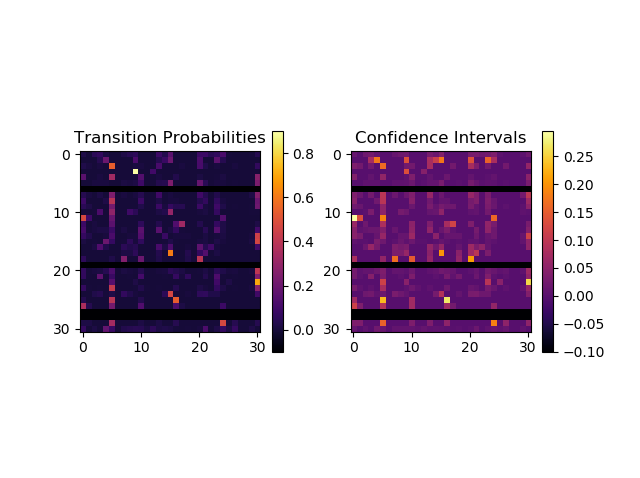
\includegraphics[width = 160mm]{Figures/Figure1.png}
	\caption{The left plot is the Transition probability matrix where 0-30 is the German alphabet and space at the end for a total of 31 characters. The right plot are the $\pm$ confidence intervals of the transition probability matrix in fractions of 1. As we can see the line at approximately 5 in the x axis of the left plot has much larger values. This character is "e" and is clearly one of the most common letter in the German alphabet which is no surprise since this is also the case in English and both are Germanic languages. The bright dot on the left plot in the top-left corner is c $\rightarrow$ h. Which is also extremely common in German since it is in many common German words. The characters that don't appear in the text have been given a confidence interval of -0.1 and transition probability of -0.1 for visual identification(black bars) because it's otherwise not possible to represent graphically but obviously their true value is simply undefined. However, to be clear no values are negative except for characters that never appeared at all, it is simply for visualization purposes. The x axis and y axis are the characters as given in Tables 1-8.}
	\label{fig:Figure1}
\end{figure}

Overall, all of the characters that appear have smaller confidence intervals than their value. Except for characters that did not appear in the text at all. In order to get good values for these we would of course need much larger texts. Or better yet, a varied selection of texts if we want a representative sample of German language texts. Since, for example, this text is relatively archaic given that it was first written by the Brothers Grimm in 1812-1822. However, it is difficult to find a text of much larger size in an accessible format since most books would be in the PDF format rather than in a simple text format. Since this assignment is not an exercise in computationally extracting text from a PDF file into a more useful format I will not choose a different text since it is already about 1500 words long. However, we can find a theoretical text size necessary for good accuracy by taking \eqref{eq:CI} and rearranging for n. Since p is some constant value for each character over the entire population of german texts. Then we can find exactly the number of occurrences of that character needed to ensure a specific confidence interval. In order to do this we can simply analyse a wide variety of different text types and size for occurrences of characters and calculate n for the least likely to occur character and take that for the total sum of text lengths necessary to ensure all confidence intervals are below some level. \\


\begin{gather}
\label{eq:CI}
	\textrm{Confidence Interval} = 1.96\sqrt{\frac{p(1-p)}{n}} \\
	\textrm{Where p is the transition probability and n is the number of occurrences of a in a $\rightarrow$ b.} \notag
\end{gather}

\newpage
\section{Task 4 - Vowels and Consonants}

% Table generated by Excel2LaTeX from sheet 'Task4Table1'
\begin{table}[htbp]
	\centering
	\caption{Transition Probabilities}
	\begin{tabular}{lrrr}
		Row $\rightarrow$ Col & \multicolumn{1}{l}{Vowels} & \multicolumn{1}{l}{Consonants} & \multicolumn{1}{l}{Space} \\
		Vowels     & 1.25E-01 & 7.48E-01 & 1.27E-01 \\
		Consonants     & 4.23E-01 & 3.01E-01 & 2.67E-01 \\
		Space & 2.74E-01 & 7.24E-01 & 8.22E-04 \\
	\end{tabular}%
	\label{tab:Task4_Transition}%
\end{table}%

% Table generated by Excel2LaTeX from sheet 'Task4Table2'
\begin{table}[htbp]
	\centering
	\caption{Confidence Intervals}
	\begin{tabular}{lrrr}
		Row $\rightarrow$ Col & \multicolumn{1}{l}{Vowels} & \multicolumn{1}{l}{Consonants} & \multicolumn{1}{l}{Space} \\
		Vowels     & 1.52E-02 & 3.70E-02 & 1.52E-02 \\
		Consonants     & 2.14E-02 & 1.80E-02 & 1.70E-02 \\
		Space & 2.94E-02 & 4.78E-02 & 1.61E-03 \\
	\end{tabular}%
	\label{tab:Task4_CI}%
\end{table}%
Tables \ref{tab:Task4_Transition} and \ref{tab:Task4_CI} were generated using the below code. Which is largely the same as in Task 2.\\
\lstinputlisting[language=Python,style = PythonStyle,firstline = 133,lastline = 169]{Code/Code.py}
 
 
\section{Task 5 and 6 - Random String}

The algorithm to generate a random string is simple. Since the transition matrix is right stochastic the sum of the rows equals to 1. Therefore we can take the probability matrix and make a new matrix containing the sum of the probabilities from the left most column to each column position and then compare values generated by a uniform distribution random number generator to the matrix with the sum of probabilities. Because if it's less than one sum of probabilities value but more than the previous value we know which character to select. The code below shows how it was done. The exact same algorithm can be used for Task 5 and 6. The code uses integers to represents characters throughout and then replaces them at the end because the integers are easier and more efficient to work with. This is not necessary but merely a choice. For Task 6, the first character was selected as e as from Task 2 we can see that it is by far the most likely to exist character and for Task 5 I started with a consonant as that is also more probable than a vowel as the first character. There are no special characters in the generated text, because all transition probabilities were calculated after stripping out the symbols. So in order to do so I would need to generate considerably more transition probabilities that wouldn't be particularly accurate considering punctuation doesn't appear as frequently and can only ever exist at the end of the word. Which these character based Markov chains cannot do. One would have to do the analysis with words to add punctuations in any feasible manner. 

\lstinputlisting[language=Python,style = PythonStyle,firstline = 174,lastline = 217]{Code/Code.py}
Where Result3[0] and Result2[0] are the transition probabilities from Task 4 and 2 respectively. \\
\bigskip
An example of the result for a randomly generated 100 character vowel-consonant-space spaghetti is
"babaaab bb b bbabb aba b ba aababbab b babbbbbb b b bb b bab babaaba abaab abbabab bbbbaababbabbabba"
which seems reasonable qualitatively. Since nothing is too long, there are quite a lot of short words, and vowels and consonants are mixed throughout. \\
\newline
An example for the result of Task 6 is, \\
"eitamein dein wie heren o upieunhe jah ste ze dahäte fen ine damman d z a niter tr d nengieieder m aunnfein hes einspfzer flonen gaune wale m warwiechn kben derchöhorichavordichaße faur des us je h imu sten we s dldan hoprt onnteicht jute könde venge aber dendafro f scherte dongichönseronden voß daberaspr efämebe im e n din un eier wuner u wähäm u d dagesess u ue ju d dachr unickerorenenie gigen dch abeinde geigen jas t tebe dr kön f gr kön sch s dah kenhetelcheröh enichöniche olltrlahterin wahnd gender d ser f d sterneick m e e den s sal ingein eflten ver doßtatestter ustr ster dandauspr hen d d in denstes gen le ihe d leihndiendam pr kr alam tteichero wämmihn de wondandie itenirende meninuf hr n ichwe dillesprlicher uspigendachten ditenmäun d hn wa st ers s aß d deund wöher die kar d s e waaasefiend miche daßtenura d usopf nefr he wön dertelten ate e de ge ster krt wat un pf wöspate ien ten den siert d wont saurn unihäten e en könafar wöleien hn end htodescheit ein sin mich galen der"

\bigskip
Qualitatively, this seems reasonable. No characters that didn't appear in the text appeared. The word lengths generally seem more or less reasonable. Single character words are too frequent since a single character word doesn't exist in German. Some if it is almsot readable and in fact some words such as "dein", "wie" , "den", "mich", "der", "scherte", "eier" are all actual german words. Which is a lot more than would be expected from a purely randomly generated text. Of course, most words are meaningless and the text doesn't make any actual sense. But that's where one would use many, much larger texts to do the same analysis but using words. At which point it would be readable but sentences probably wouldn't make sense in general. So the main difference, is that it doesn't make any sense whatsoever unlike an actual text.  
\clearpage
\printmybibliography
\end{document}